\chapter*{Foreword}
\markboth{Foreword}{Foreword} 
%\lhead{\emph{Foreword}}
\label{chap:foreword}
\begin{chapquote} {Miro Astore}
Choose some nice and fun chapter quotes, they're the most fun thing about writing a thesis
\end{chapquote}

Good luck!

%this is a really nice way to format figures I like, it means you can make captions as long as you like. 
%\begin{figure}[h]
%	\begin{center}
%		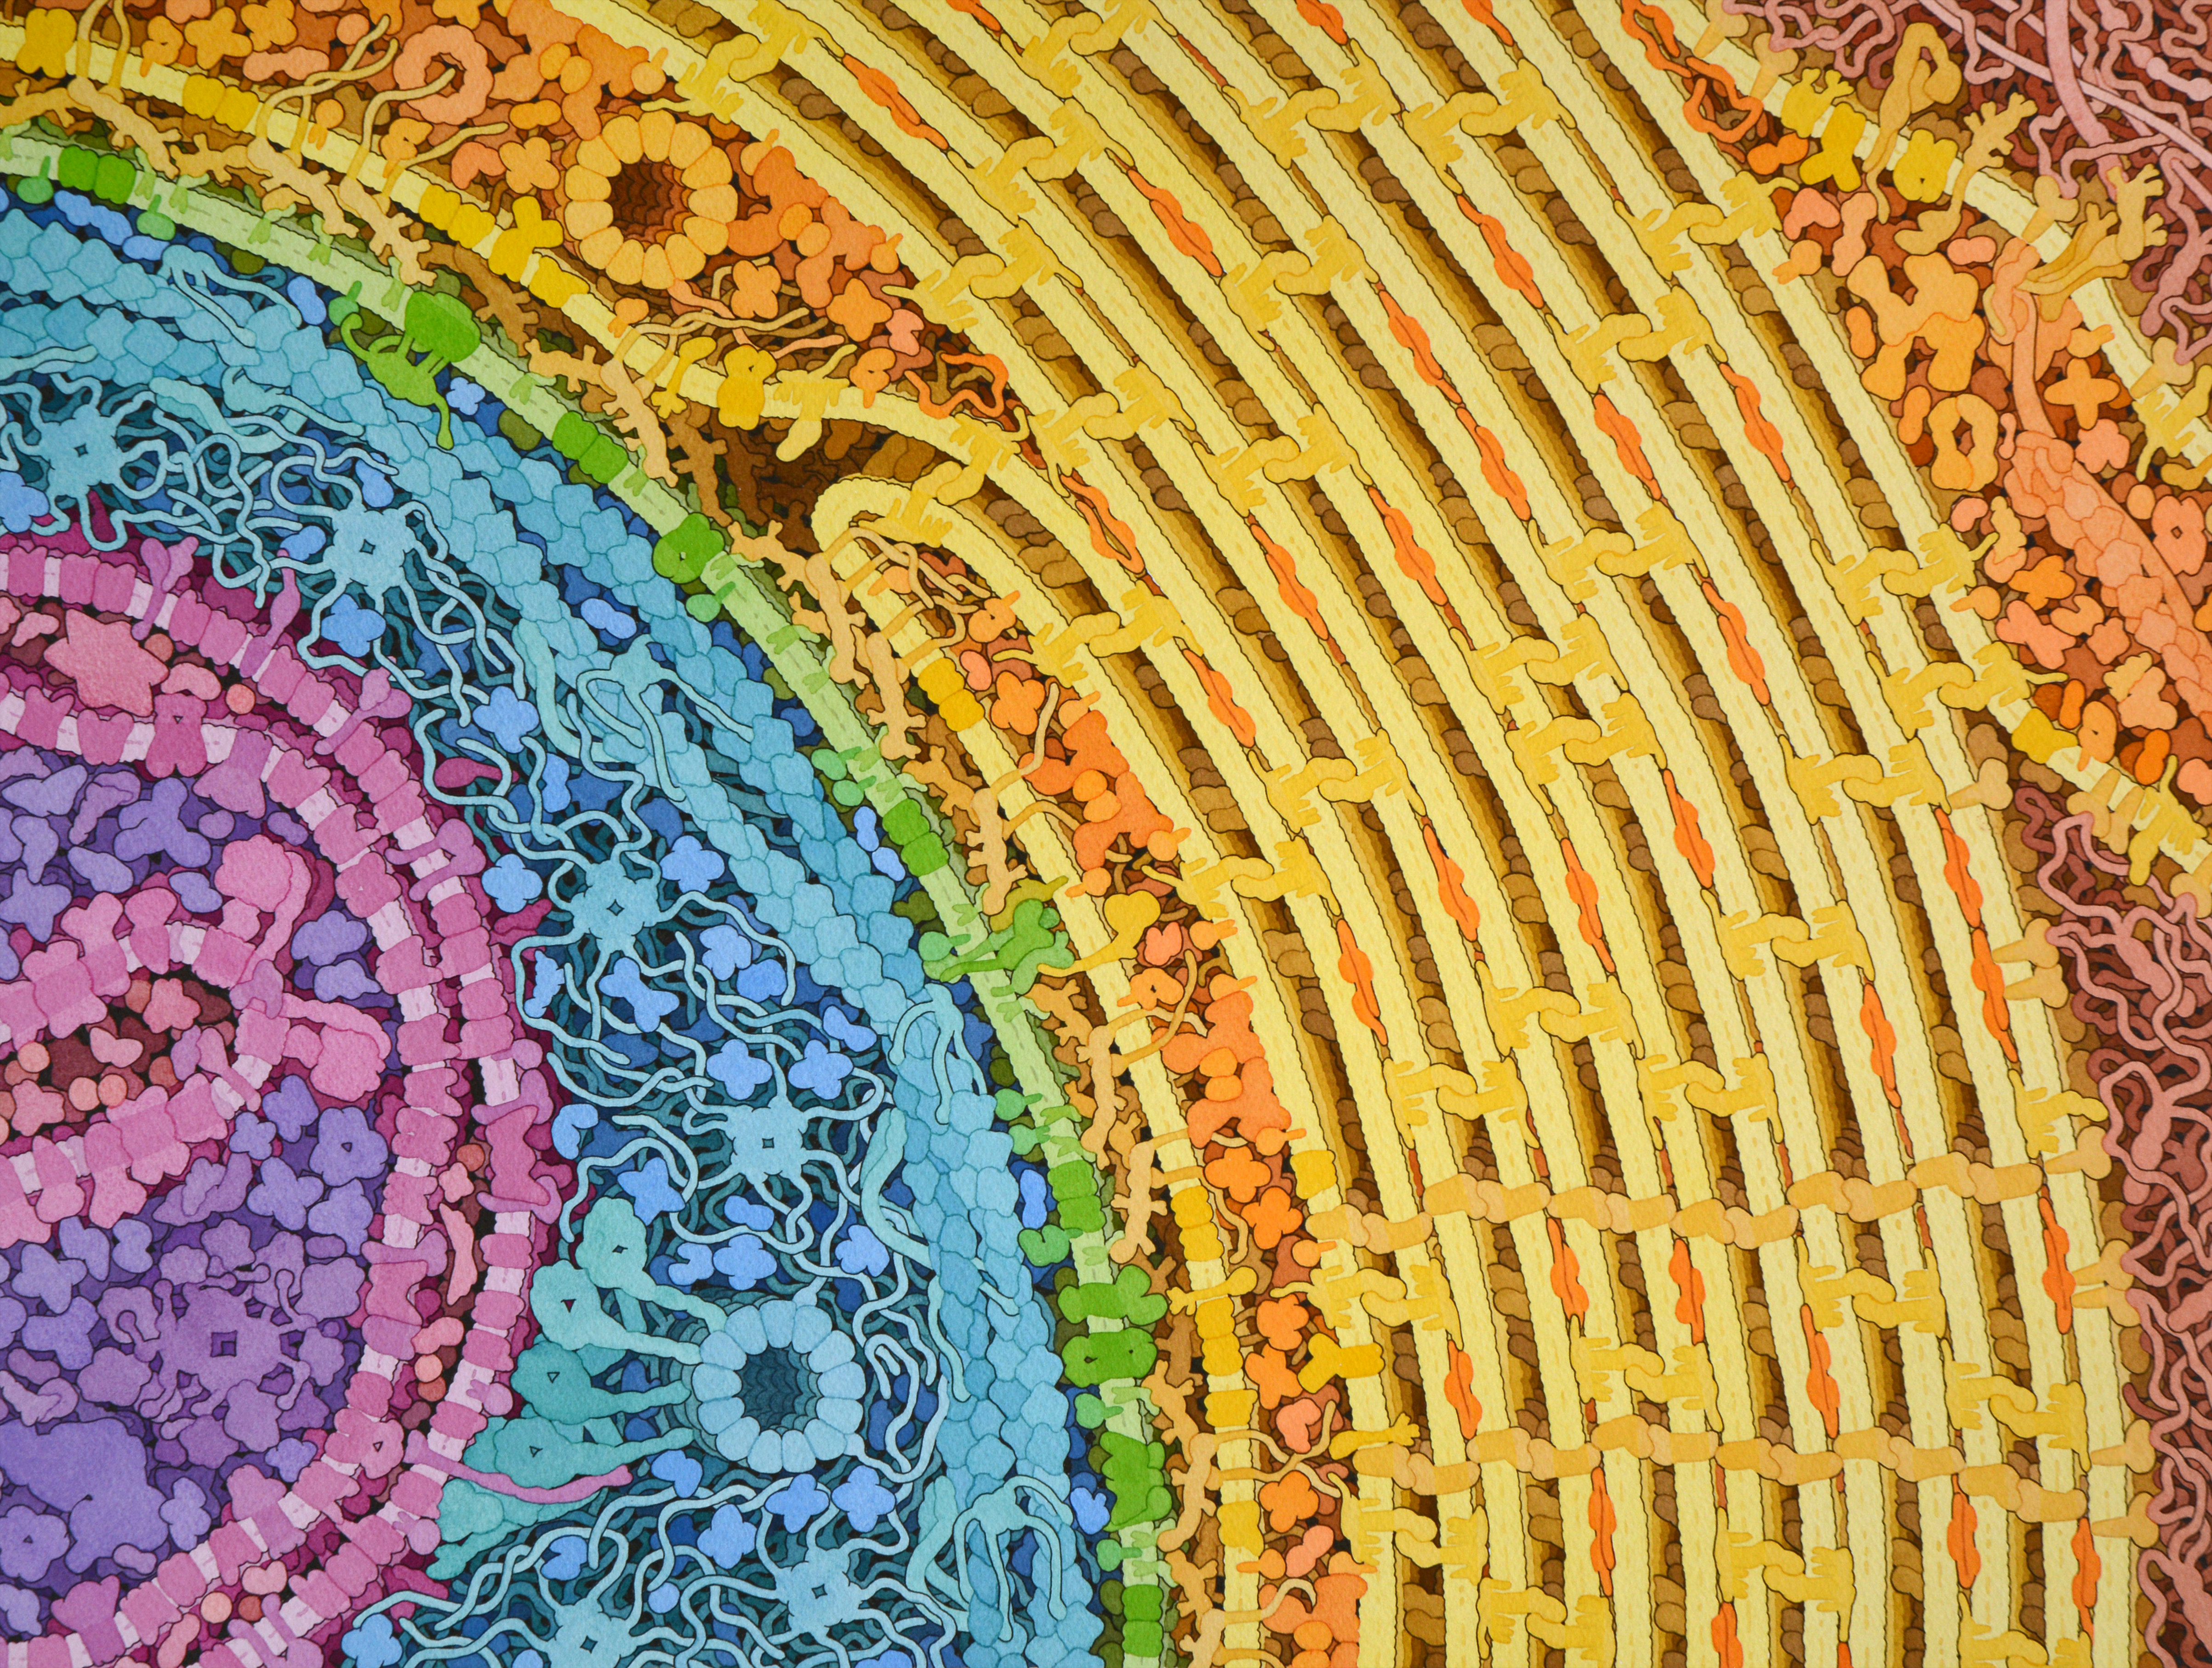
\includegraphics[width=0.9\textwidth]{figures/myelin.jpg}
%	\end{center}
%	\captionsetup{singlelinecheck = false, justification=raggedright}
%	\caption[Nerve Cross Section by David Goodsell] {\textbf{Nerve Cross Section by David Goodsell}}{David Goodsell is an artist who produces water paintings of cellular environments. Many of his works can be downloaded and used \href{https://pdb101.rcsb.org/sci-art/goodsell-gallery}{for free}. He has also written many books and articles which would serve as a light, layperson friendly introduction to molecular biology \cite{goodsell2009, goodsell2018, goodsell2020}. This particular painting depicts the cross section of a nerve. The nerve fibre (blue) is wrapped in an insulating myelin sheath (yellow). Electrical signals propagate perpendicular to the page, via voltage gated sodium and potassium protein ion channels at the edge of the nerve\cite{goodsell_nerve}. We will discuss the discovery and details of this mechanism in the next chapter, as they were critical to the development of biophysics.}
%	\label{goodsell_figure}
%\end{figure}

